\documentclass[12pt]{exam}

\usepackage{amssymb}
\usepackage{mathtools}
\usepackage{algorithm}
\usepackage{float}  % Figure placement
\usepackage{minted}  % Code highlighting
\usepackage{tikz}  % Flow chart
\usepackage{lipsum}
\usepackage{xspace}
\usepackage{hyperref}
\usepackage{MnSymbol}
\usepackage{pgffor}


\hypersetup{
    colorlinks = true,
    linkcolor = blue,
    urlcolor  = blue,
    citecolor = blue,
    anchorcolor = blue
}

\newcommand{\hwheaderfooter}[3]{
\pagestyle{headandfoot}
\firstpageheadrule
\firstpageheader{#1}{#2}{#3}
\runningheader{#1}{#2}{#3}
\runningheadrule
\firstpagefooter{}{\thepage}{}
\runningfooter{}{\thepage}{}
}

\newcommand{\latex}{\LaTeX\xspace}

\newcommand{\stars}[1]{%
    \foreach \n in {1,...,#1}{%
        $\filledstar$%
    }%
}

\usetikzlibrary{shapes.geometric, arrows}
\tikzstyle{arrow} = [thick,->,>=stealth]

\hwheaderfooter{HW 2}{Ching}{CSCI 406}


\begin{document}
\begin{center}
    \fbox{\fbox{\parbox{\textwidth - 0.2 in}{\centering

                {Instructions: Please note that handwritten assignments \textbf{will not be graded}. Use the
                    provided \latex template to complete your homework. Please do not alter the order or spacing of
                    questions (keep each question on its own page). When you submit to Gradescope, you must mark
                    which page(s) correspond to each question. \textbf{You may not receive credit for unmarked
                        questions}. \\ When including graphical figures, we encourage the use of tools such as \href{https://dreampuf.github.io/GraphvizOnline/}{graphviz} or packages like \href{https://www.overleaf.com/learn/latex/TikZ_package}{tikz} for simple and complex figures. However, these may be handwritten only if they are neat and legible (as defined by the grader). }\\

            }}}
\end{center}

\textbf{List any collaborators (besides TAs or professors) here:}

\begin{questions}

    \question[35] [Maze, \stars{5}] Describe the graph model for Spacewreck. How will you encode the complexities and rules of the game into a graph? You must be able to run an \textbf{unmodified} BFS to find the shortest sequence of moves for either Captain Rocket or Lieutenant Lucky to reach the Goal. In order for BFS to work, your model must have exactly one start vertex and exactly one finish vertex.


    \textbf{Graph Model}

    Vertex - possible game states (room location of each person)\\
    Edge - possible moves to new game states \\

    Each iteration of BFS will add all possible moves from the current game state to the queue. \\
    BFS will terminate when either Captain Rocket or Lieutenant Lucky reaches the goal. \\
    BFS will return the path from the start vertex to the goal vertex.


    This handles things like loops, because BFS will not add a game state to the queue if it has already been visited allowing it to exit the failed path and continue searching


    \clearpage

    \question[5] [W3, \stars{1}] For the following questions, select whether the statement is true or false,
    and write a \textit{brief} explanation of your reasoning.

    \begin{parts}
        \part Topological Sort results in a unique ordering

        % Replace \square with \blacksquare for the option you would like to select.
        $\square$ True $\blacksquare$ False

        While a topological sort guarantees precedence is followed, it is not guaranteed to be unique. For example, the graph below has two possible topological sorts: $1, 2, 3, 4$ and $1, 3, 2, 4$.

        \begin{figure}[H]
            \centering
            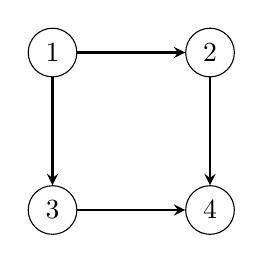
\begin{tikzpicture}[node distance=2cm]
                \node (1) [circle, draw] {1};
                \node (2) [circle, draw, right of=1] {2};
                \node (3) [circle, draw, below of=1] {3};
                \node (4) [circle, draw, right of=3] {4};

                \draw [arrow] (1) -- (2);
                \draw [arrow] (1) -- (3);
                \draw [arrow] (2) -- (4);
                \draw [arrow] (3) -- (4);
            \end{tikzpicture}
        \end{figure}

        \part It is impossible to find a topological ordering on a cyclic graph.

        % Replace \square with \blacksquare for the option you would like to select.
        $\blacksquare$ True $\square$ False

        A topological ordering is only possible on a DAG. A cyclic graph is not a DAG, so it is impossible to find a topological ordering on a cyclic graph.

    \end{parts}

    \clearpage

    \question[20] [W2/3, \stars{2}]
    In BFS and DFS, an undiscovered node is marked \textit{discovered} when it
    is first encountered, and marked processed when it has been completely searched.
    At any given moment, several nodes might be simultaneously in the
    \textit{discovered} state.

    \begin{parts}
        \part[7] Describe a graph with $n$ vertices such that $n - 1$ vertices are simultaneously in the discovered state at some point during a \textbf{BFS} from a starting vertex $v$ of your choosing.

        A star graph where $v$ is the center vertex and each branch had the same depth. For example, the graph below is a star of 6 vertices, where 5 vertices are simultaneously in the discovered state at some point during a \textbf{BFS} from a starting vertex $1$.

        \part[3] Draw a graph with $n=6$ vertices that matches the description in part (a). Clearly indicate which vertex is the starting vertex.

        Gray = discovered, white = undiscovered, black = processed.
        \begin{figure}[H]
            \centering
            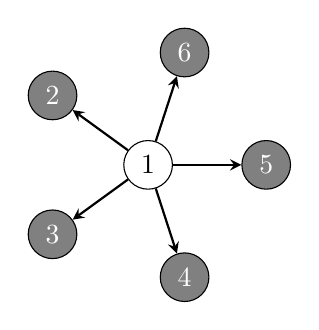
\begin{tikzpicture}
                % Nodes forming a star
                \node[circle, draw] (N1) at (0,0) {1};

                % Nodes forming a complete graph
                \foreach \i in {2,...,6}
                \node[circle, draw, fill=gray, text=white] (N\i) at (72*\i:1.5) {\i};

                % Edges for the complete graph
                \foreach \i in {2,...,6}
                \draw [arrow] (N1) -- (N\i);
            \end{tikzpicture}
        \end{figure}

        \part[7] Describe a graph with $n$ vertices such that $n - 1$ vertices are simultaneously in the discovered state at some point during a \textbf{DFS} from a starting vertex $v$ of your choosing.

        A linear graph in which $n$ vertices form a list, where $n \geq 2$. For example, the graph below is a line of 6 vertices, where 5 vertices are simultaneously in the discovered state at some point during a \textbf{BFS} from a starting vertex $1$.

        \part[3] Draw a graph with $n=6$ vertices that matches the description in part (b). Clearly indicate which vertex is the starting vertex.

        Gray = discovered, white = undiscovered, black = processed.
        \begin{figure}[H]
            \centering
            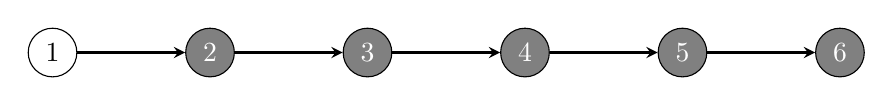
\begin{tikzpicture}[node distance=2cm]
                \node (1) [circle, draw] {1};
                \node (2) [circle, draw,fill=gray, text=white, right of=1] {2};
                \node (3) [circle, draw,fill=gray, text=white, right of=2] {3};
                \node (4) [circle, draw,fill=gray, text=white, right of=3] {4};
                \node (5) [circle, draw,fill=gray, text=white, right of=4] {5};
                \node (6) [circle, draw,fill=gray, text=white, right of=5] {6};

                \draw [arrow] (1) -- (2);
                \draw [arrow] (2) -- (3);
                \draw [arrow] (3) -- (4);
                \draw [arrow] (4) -- (5);
                \draw [arrow] (5) -- (6);
            \end{tikzpicture}
        \end{figure}

    \end{parts}

    \clearpage

    \question[10] [W2/3, \stars{2}] Your friend Alice has recently returned from a trip to a wonderful land. While describing her adventures, she tells you about a curious hedge maze she encountered. ``The maze went on and on forever,'' she tells you. ``I don't think it had an end!'' Fortunately, a friendly cat directed her to the exit.

    This strange tale has you thinking about infinite mazes. \textbf{Which of the following statements are true about searching infinite mazes (graphs) where all nodes have \textit{finite} degree?}

    Assume the following about the infinite maze:
    \begin{itemize}
        \item the maze has a single connected component and that we are starting from a start location and searching for an end location that exists somewhere \textbf{in} the maze,
        \item there is a finite distance between the start and end locations, and
        \item we stop the traversal once the end location is reached.
    \end{itemize}

    $\blacksquare$ A DFS may never terminate. \\
    $\blacksquare$ A BFS may never terminate.

    DFS and BFS will never terminate on an infinite cyclic graph.

    $\blacksquare$ A DFS might terminate, but the solution may not be the shortest path.

    DFS only guarantees the shortest path on a tree.

    $\blacksquare$ A BFS might terminate, but the solution may not be the shortest path.

    BFS only guarantees the shortest path on unweighted, finite graphs.

    $\square$ A DFS will terminate, and the solution will be the shortest path. \\
    $\square$ A BFS will terminate, and the solution will be the shortest path.

    DFS and BFS are not guaranteed to terminate on infinite graphs.


    \clearpage

    \question[30] [W2/3, \stars{4}] A primary application of BFS is finding shortest paths in an unweighted graph. Consider a weighted graph with edges of cost 0 and 1. Describe how to modify the BFS algorithm to find the shortest path between two vertices in this type of graph. The worst case complexity must remain the same ($\mathcal{O}(V + E)$).

    \textbf{Modification:} Instead of using a queue, use a double-ended queue. When adding a vertex to the queue, add it to the back if the edge has weight 1, and add it to the front if the edge has weight 0. This ensures that the shortest path is found first.

    \textbf{0-1BFS}

    Initialize a double queue $Q$ and a parent array $P$. \\
    Enqueue the start vertex $s$ into $Q$ and set $P[s] = NULL$. \\
    While $Q$ is not empty: \\
    \hspace*{1cm} Dequeue the front vertex $u$ from $Q$. \\
    \hspace*{1cm} For each neighbor $v$ of $u$: \\
    \hspace*{2cm} If $P[v]$ is undefined: \\
    \hspace*{3cm} Set $P[v] = u$. \\
    \hspace*{3cm} If the edge $(u, v)$ has weight 0: \\
    \hspace*{4cm} Enqueue $v$ at the front of $Q$. \\
    \hspace*{3cm} Else: (weight of 1)\\
    \hspace*{4cm} Enqueue $v$ at the back of $Q$. \\
    Return $P$.
    % close the document
\end{questions}
\end{document}
